\documentclass{beamer}

\mode<presentation> {

    \usetheme{Madrid}
    \usecolortheme{beaver}
}


\usepackage{graphicx}


%--------------------------------------------------
% Macros
%--------------------------------------------------
\newtheorem{command}[theorem]{Command}

%--------------------------------------------------
% Title Page
%--------------------------------------------------

\title[git]{A short introduction to git}
\author{John Ladan}
\institute[Waterloo]{University of Waterloo\\john@ladan.ca}
\date{\today}

\begin{document}

\begin{frame}
    \titlepage
\end{frame}

\begin{frame}
    \frametitle{Overview}
    \tableofcontents
\end{frame}

%--------------------------------------------------
% Presentation slides
%--------------------------------------------------

\section{What is git?}

\begin{frame}
    \frametitle{According to git-scm.com}
    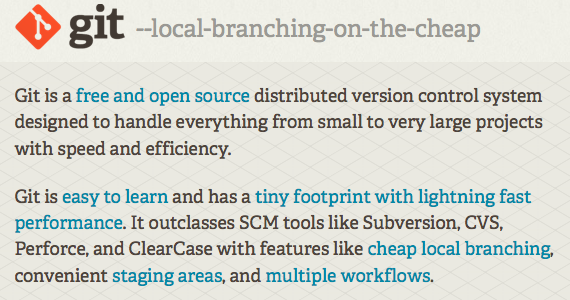
\includegraphics[width=.8\textwidth]{figures/git-homepage}
\end{frame}

\begin{frame}
    \frametitle{According to wikipedia.org}
    Git (/ɡɪt/) is a distributed revision control system with an emphasis on speed, data integrity, and support for distributed, non-linear workflows. Git was initially designed and developed by Linus Torvalds for Linux kernel development in 2005, and has since become the most widely adopted version control system for software development.

    As with most other distributed revision control systems, and unlike most client–server systems, every Git working directory is a full-fledged repository with complete history and full version-tracking capabilities, independent of network access or a central server. Like the Linux kernel, Git is free software distributed under the terms of the GNU General Public License version 2.
\end{frame}

\begin{frame}
    \frametitle{Features}
    \begin{itemize}
        \item Fast
        \item Nonlinear development (via rapid branching, and DAG based structure)
        \item Distributed -- each copy of the repo is complete by itself
            \begin{itemize}
                \item each copy of the repo is itself a repo
                \item changes can be pushed/pulled to any other instance
                \item do not need network access
            \end{itemize}
        \item Ubiquitous
        \item Good \emph{free} repository hosting (github)
    \end{itemize}
\end{frame}

\section{More detail}


\begin{frame}
    \frametitle{Structure of a repository}
    \begin{itemize}
        \item Everything is stored in files, with all the metadata (esp. history) in \texttt{.git}.
        \item The history is structured as a Directed Acyclic Graph (DAG). It's basically just a tree where branches can join back together.
        \item The history is (for the most part) stored as changes (diffs) between the nodes (commits). 
    \end{itemize}
\end{frame}

% show an example of a repo here.

\begin{frame}
    \frametitle{Git Terminology}
    A few terms to help you out.
    \begin{itemize}
        \item Commit: \emph{n}. A particular snapshot of the project, labelled with a unique hash.
        \item remote: \emph{n}. A remote repository that should have the same commit history (to a point)
        \item branch: \emph{n}. A pointer to a specific commit. When the branch is checked out, commiting changes will advance that pointer.
        \item master: the main branch of the repository
        \item merge: \emph{v}. The process of combining two branches
        \item rebase: \emph{v}. cutting of a branch, and grafting it on somewhere else.
        \item HEAD: \emph{n}. The currently checked out commit.
        \item tag: \emph{n}. A fancy branch label that stays put, and can be signed by the author
    \end{itemize}
\end{frame}

\section{Cloning a Repo}

\begin{frame}
    \frametitle{Basic workflow}
    \begin{itemize}
        \item clone/create a repository
        \item branch
        \item make changes
        \item commit
        \item merge changes into main branch
        \item push changes upstream
    \end{itemize}
\end{frame}

\begin{frame}
    \frametitle{Git Clone}
    \begin{command}
        \texttt{git clone <repository-location> [<local-path>]}
    \end{command}
    It's a lot like downloading a tarball, except
    \begin{itemize}
        \item only the necessary files are included (no build files)
        \item lots of option, like pulling a specific commit, or not downloading full history
    \end{itemize}
\end{frame}

\begin{frame}
    \frametitle{Submodules}
    Word of warning: some packages use \emph{submodules}. One way to handle it:
    \begin{command}
        \texttt{git clone --recursive <repo>}
    \end{command}
\end{frame}

\section{Making Changes}

\begin{frame}
    \frametitle{Branching}
    You should always branch first:
    \pause
    \begin{itemize}
        \item it's a good habit to be in;
        \item the last good state is left labeled;
        \item easy to checkout other branches, even when you're in the middle of something;
        \item pulling origin/master is easier; and
        \item branches are cheap!
    \end{itemize}
\end{frame}

\begin{frame}
    \frametitle{Git Branch}
    \begin{command}
        \texttt{git branch <branch-name>}\\
        \texttt{git checkout <branch-name>}
    \end{command}
    Alternatively,
    \begin{command}
        \texttt{git checkout -b <branch-name>}
    \end{command}
\end{frame}


\begin{frame}
    \frametitle{Editing}
    When editing, you can use whatever tools you want, with one (or two) exceptions:
    \pause
    moving and removing files.
    \begin{command}
        \texttt{git mv <file> <new-filename>}
    \end{command}
    \begin{command}
        \texttt{git rm <file>}
    \end{command}
    This way, git understands that it is the same file (or that it is intentionally gone).
\end{frame}


\section{Commiting Changes}

\begin{frame}
    \frametitle{Seeing your changes}
    Before committing, it's a good idea to see what changes you made
    \begin{command}
        \texttt{git status}
    \end{command}
    \pause
    And if you want the details,
    \begin{command}
        \texttt{git diff <file>}
    \end{command}
\end{frame}

\begin{frame}
    \frametitle{Staging files}
    Next, we need to let git know what files have changed, and what new files it should track
    \begin{command}
        \texttt{git add <file(s)>}
    \end{command}
    \pause
    Often, it's good to check the \emph{status} again before the next step
\end{frame}

\begin{frame}
    \frametitle{Commit!}
    Finally, we commit our changes to the tree.
    \begin{command}
        \texttt{git commit [-m "Message text"]}
    \end{command}
    \pause
    (I recommend not using the \texttt{-m} flag)
\end{frame}


\begin{frame}
    \frametitle{Practice safe committing}
    Here are a few best practices:
    \begin{itemize}
        \item Commits should be small and non-breaking
        \item The message should complete the sentence ``This commit will...''
        \item Keep the commit to one feature/bug-fix
        \item Don't use the \texttt{-m} flag
    \end{itemize}
\end{frame}

\begin{frame}
    \frametitle{Speeding up commits}
    There's a faster way...
    \begin{command}
        \texttt{git commit -a}
    \end{command}
    The \texttt{-a} flag stages \emph{all} modified files, but not any untracked files.
\end{frame}

\begin{frame}
    \frametitle{Merging}
    After some commits, you'll probably want to add those changes to the main branch.
    \begin{command}
        \texttt{git checkout master \\ git merge <other-branch>}
    \end{command}
    If there are no conflicts (i.e. the commit is a direct descendent), the current branch will be fast-forwarded. This just means the pointer gets moved ahead.

    If there are conflict, we have to fix them manually.
\end{frame}

\section{Sharing with others}

\begin{frame}
    \frametitle{Pushing}
    What about sending the changes upstream?
    \begin{command}
        \texttt{git push [<remote-name>]}
    \end{command}
    \pause
    If the remote branch has changed you'll have to pull first
    \begin{command}
        \texttt{git pull [<remote-name>]}
    \end{command}
    and then push.
    \pause
    Because of this, it's probably better to pull before merging your working branch. That should keep the tree of commits cleaner.
\end{frame}


\section{Rolling Your Own}

\begin{frame}
    \frametitle{Rolling your own}
    \begin{itemize}
        \item What normally happens.
        \item What ideally happens.
    \end{itemize}
\end{frame}

\begin{frame}
    \frametitle{Typical Case}
    This is what often happens...
    \begin{itemize}
        \item start coding, and realize you want this in a git repo
        \item create a new repo
    \end{itemize}
    \begin{command}
        \texttt{git init ; git add... ; git commit}
    \end{command}
    \begin{itemize}
        \item continue coding, then realize you want a remote backup
        \item create a repo on github, then...
    \end{itemize}
    \begin{command}
        \texttt{git remote add origin <repo-url>; git push -u master origin}
    \end{command}
\end{frame}


\begin{frame}
    \frametitle{Problems}
    Pros:
    \begin{itemize}
        \item you can always retroactively add version control to a project
    \end{itemize}
    Cons:
    \begin{itemize}
        \item All the past revision history is lost.
        \item These commands are more obscure and harder to remember.
    \end{itemize}
\end{frame}

\begin{frame}
    \frametitle{Ideal Case}
    \begin{itemize}
        \item Have the foresight to create a repo (e.g. on github)
        \item Clone that repo onto your workstation
        \item Start coding and commiting as usual
    \end{itemize}
\end{frame}


\begin{frame}
    \frametitle{One more thing}
    If you don't want to share your project publicly, and have access to a server,
    \begin{command}
        \texttt{git init --bare}
    \end{command}
    This creates a "headless" repo, storing all the data, but without the working tree. You can then push/pull/clone from this remote repo as usual.
    \pause

    E.g. I put all of my repos in a directory on CSC servers. \texttt{jladan@taurine.uwaterloo.ca:/users/jladan/git-repos/}
\end{frame}

\section{Version Control}

\begin{frame}
    \frametitle{Version Control}
    Now for the reasons \emph{why} we actually go through all this effort.
\end{frame}

\begin{frame}
    \frametitle{Checking out}
    Any point in the DAG can be accessed by checking it out
    \begin{command}
        \texttt{git checkout <branch-name|commit-hash>}
    \end{command}
    This changes the working tree to be in the state of that commit. However, no untracked files are changed.
\end{frame}

\begin{frame}
    \frametitle{Undo! Undo!}
    The easiest time to undo your changes is before committing them.
    \begin{command}
        \texttt{git checkout -- <filename>}
    \end{command}
\end{frame}



\begin{frame}
    \frametitle{Undo! Undo!}
    But what if you didn't mean to commit that change?
    \begin{command}
        \texttt{git reset [--hard] HEAD\~{}1}
    \end{command}
    \pause
    HEAD\~{}n is a synonym for `n commits before head'

    \pause
    \alert{Do not delete commits that are already upstream}
\end{frame}

\begin{frame}
    \frametitle{Git Reset}
    The reset command actually performs a lot of different functions. It's like the `undo' of git.

    It's probably a good idea to read the man-page for it
    \begin{command}
        \texttt{man git-reset}
    \end{command}

    There are a lot of useful recipes at the end of that document.
\end{frame}

\begin{frame}
    \frametitle{I made a mistake in that last commit!}
    If you made a mistake in what changes were staged or the commit message has a typo,
    \begin{command}
        \texttt{git commit --amend}
    \end{command}
    \pause
    \alert{This creates a new commit}. Each commit is labeled by its hash, so amending a commit actually replaces it with a new one. Thus you cannot ammend commits that have already been pushed.
\end{frame}

\begin{frame}
    \frametitle{Tagging and Versions}
    Saving the location in the tree of a specific version is easy
    \begin{command}
        \texttt{git tag <tag-name>}
    \end{command}
    A tag is essentially just a branch name that is fixed in place. It can also be signed by the developer, so that no one tampers with it later.
\end{frame}

\section{In Practice}

\begin{frame}
    \frametitle{What you'll use a lot}
    \begin{itemize}
        \item git status: tells you where you are, and what commands you might want to use
        \item git log: tells you where everything is (reminder: git glog)
        \item git commit
    \end{itemize}
\end{frame}


\begin{frame}
    \frametitle{Getting Help}
    There are 3 main sources of help for git:
    \begin{itemize}
        \item git status
        \item man pages: man git-<command>
        \item google
    \end{itemize}
    Github is also good at telling you the commands to do various things
\end{frame}

\begin{frame}
    \frametitle{github example}
    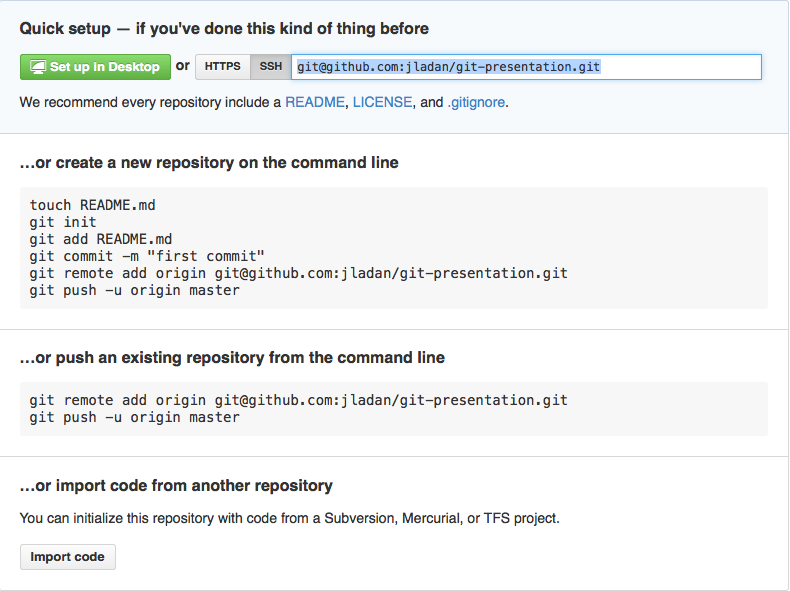
\includegraphics[height=.80\textheight]{figures/creating-on-github}
\end{frame}

\begin{frame}
    \frametitle{Other functions}
    Stashing can be quite useful when you haven't branched
    \begin{command}
        \texttt{git stash \\ git checkout -b <new-branch> \\ git stash pop}
    \end{command}

    \pause
    Rebasing can help keep the graph clean
    \begin{command}
        \texttt{git rebase <new-root>}
    \end{command}
    You can combine and reorder commits in this process too. However, some people frown on this practice, because it doesn't accurately track the history.
\end{frame}


\begin{frame}
    \frametitle{A few other things}
    \begin{itemize}
        \item You'll have to delete the old branch names from time to time
        \item To contribute to other projects, you'll likely need to do a `pull request'
        \item You should always have a license and readme file
        \item Keep a clean setup with \texttt{.gitignore}
    \end{itemize}
\end{frame}

\end{document}
